\todo{Wichtige Begriffe erklären}
\subsection{Element- und Verbindungshalbleiter}

	Zunächst wird zwischen Element und Verbindungshalbleitern unterschieden. Bei den Elementhalbleitern handelt es sich um Silizium und Germanium. Dies sind beides Halbleiter der 4. Hauptgruppe (\ref{11_perioden}). Verbindungshalbleiter werden aus einer Verbindung von Elementen der 2. bis 6. Gauptgruppe zusammengesetzt. Einige Vertreter sind z.B. Gallium-Arsenid(GaAs) als Mischung von 3. und 5. Gruppe, Cadmium-Sulfid(CdS) als Verbindung von 2. und 6. und Silizium-Carbid(SiC) aus den Gruppen 4 und 6. Es gibt auch Verbindungshalbleiter die aus einer Mischung aus Germanium und Silizium bestehen. Dies kann für verspanntes Silizium verwendet werden. 

	\begin{figure}[h]
		\centering
		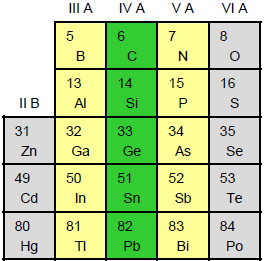
\includegraphics[width=0.5\textwidth]{Kapitel/Kap11/periodensystem.png}
		\caption{Ausschnitt der 2. bis 6. Hauptgruppe des Periodensystems der Elemente}
		\label{11_perioden}
	\end{figure}

	Die Struktur entspricht einem Diamantgitter. Sie tritt sowohl bei Element, als auch bei Verbindungshalbleitern auf. Bei letzteren wird sie allerdings auch Zinkblende-Struktur genannt.

	\subsubsection{Direkte und indirekte Halbleiter}
	Direkte und indirekte Halbleiter unterscheiden sich in der Position des Minimums / Maximums im Bänderdiagramm. Bei direkten Halbleitern ist ein Übergang vom Valenz in das Leitungsband direkt möglich. Bei indirekten hingegen muss neben der direkten Energiedifferenz auch eine Änderung des Impuls erfolgen (\ref{11_vergleich}). Dieses benötigt allerdings viel Energie, weshalb optische Bauelement, die z.B. leuchten sollen, nur aus direkten Halbleitern gebaut werden können. Die Energie, die für einen indirekten Übergang notwendig wären, liegen nicht mehr im für uns sichtbaren Licht.
	
	\begin{figure}[h]
		\centering
		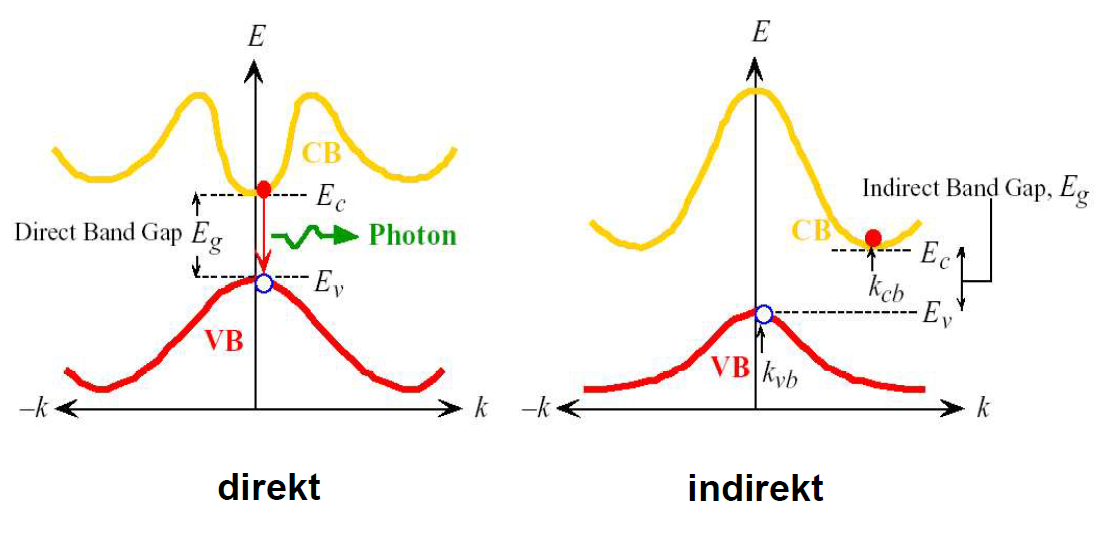
\includegraphics[width=0.8\textwidth]{Kapitel/Kap11/direkte_indirekte_halbleiter.PNG}
		\caption{Direkter und indirekter Halbleiter im Vergleich}
		\label{11_vergleich}
	\end{figure}

	\begin{table}[h]
		\centering
		\begin{tabular}{c|c|c}
			&Direkt & Indirekt \\
			\hline
			EVB(max) und ELB(min) bei & gleichem k & verschiedenen k \\
			Impulsänderung beim Übergang & nein & notwendig \\
			Übergangs- und damit Rekombinationswahrscheinlichkeit & hoch & niedrig \\
			Lebensdauer angeregter Ladungsträger & kurz & lang\\
			Optoelektronik(LED, Laser usw.) & ja & nein\\
		\end{tabular}
		\caption{Unterschiede Direkter und indirekter Halbleiter}
		\label{11_unterschiede}
	\end{table}
	
	\subsubsection{Dotieren von Verbindungshalbleitern}	
	Das Dotieren von Elementhalbleitern ist relativ einfach. Bei Verbindungshalbleiter ist dies aber nicht so. Nehmen wir das Beispiel GaAs. Hier wird z.B. mit Silizium und Kohlenstoff dotiert. Ersetzt ein Si-Atom ein Ga-Atom, so komm es zu einer n-Dotierung. Ersetzt es hingegen ein As-Atom, so ist dies eine p-Dotierung. Dies ist jedoch technische schwer umzusetzen. Einfach ist es, wenn kleinere Atome nur größere ersetzten. Eine p-Dotierung wäre mit Kohlenstoff-Atomen möglich, ist aber oftmals schwieriger.
	
	\paragraph{Antiphasengrenze} Bei Verbindungshalbleitern tritt ein neuer Defekt auf. Möchte man z.B. GaAs auf eine Siliziumoberfläche aufbringen, kann es passieren, dass durch Unebenheiten des Siliziums Antiphasengrenzen im ausgetragenen Halbleiter entstehen (\ref{11_antiphase}).
	
	\begin{figure}[h]
		\centering
		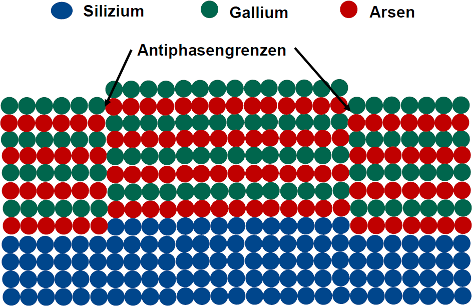
\includegraphics[width=0.5\textwidth]{Kapitel/Kap11/antiphasen.png}
		\caption{Antiphasengrenzen im GaAs}
		\label{11_antiphase}
	\end{figure}
	
	\subsubsection{Ladungsträgerbeweglichkeiten}
	
	Die Ladungsträgerbeweglichkeiten unterscheiden sich in Unterschiedlichen Materialien stark (\ref{11_ladung}). So hat GaAs eine erheblich höhere Beweglichkeit von Elektronen, die von Löchern ist allerdings noch niedriger als die von Silizium. 
	\begin{table}[h]
		\centering
		\begin{tabular}{c|c|c}
			& $\mu_n $ & $\mu_p$ \\
			\hline
			Si & 1430 & 505 \\
			Ge & 3900 & 1900 \\
			GaAs & 8000 & 400 \\
			Cu & 32 & -\\
		\end{tabular}
		\caption{Ladungsträgerbeweglichkeit in unterschiedlichen Materialien}
		\label{11_ladung}
	\end{table}
	\paragraph{HEMT} \todo{Coming soon}
\subsection{Welleneigenschaften}
	\subsubsection{Monochromatisch}
	Monochromatisches Licht besteht nur aus einem einzigen spektralen Anteil. Somit das das Licht eine bestimmte Energie. Es ist sozusagen gleichfarbig.
	\subsubsection{kohärent} 
	Kohärenz bedeutet Phasengleichheit. Dies ist vor allem dann wichtig, wenn es zu Interferenz kommen soll. Ein guter Laser erzeugt kohärentes Licht. 
	\subsubsection{kollimiert}
	Bei kollimierten Licht verlaufen alle Lichtstrahlen parallel zueinander. Dies ist zum Beispiel bei einem Laser der Fall. Generelle geht man davon aus, dass auch unser Sonnenlicht kollimiert ist, da die Sonne eine derartig große Distanz zu uns aufweist, dass die Strahlen auf der Erde nahezu parallel ankommen.


\subsection{Leuchtdioden}
	\subsubsection{Funktionsprinzip}
	
	\paragraph{Aufbau} LEDs besitzen einen Napf, in dem einen Stück Halbleitermaterial eingebunden ist. Dieser Napf ist mit einem der beiden Pole verbunden und kann von außen angeschlossen werden. Der andere Pol wird über einen dünnen Bonddraht verbunden. Der gesamte Aufbau ist in Plastik eingegossen.
	
	\paragraph{Funktion} Bei dem Halbleitermaterial handelt es sich um einen pn-Übergang. Dabei ist die p-Schicht sehr löcherreich, dünn und auf der oberen Seite. Wird nun in Durchlassrichtung eine Spannung angelegt und ist diese groß genug, um die Bandlücke zu überwinden, so kommt es zu einer Überschwemmung der Grenzschicht mit freien Ladungsträgern. Bei der Rekombination (\ref{11_rekombination}) dieser wird Licht abgestrahlt. Dabei sollte es jedoch nur zur strahlenden Rekombination kommen. Auger, Störstellen und Oberflächenrekombination sollte weitestgehend vermieden werden. Die Helligkeit kann durch die Stromstärke geregelt werden. Wird sie zu heiß, kann sie ausfallen. Da die Farbe von der Bandlücke abhängt, gibt es für verschiedene Farben verschiedene Schwellspannungen.
	
	\begin{figure}
		\centering
		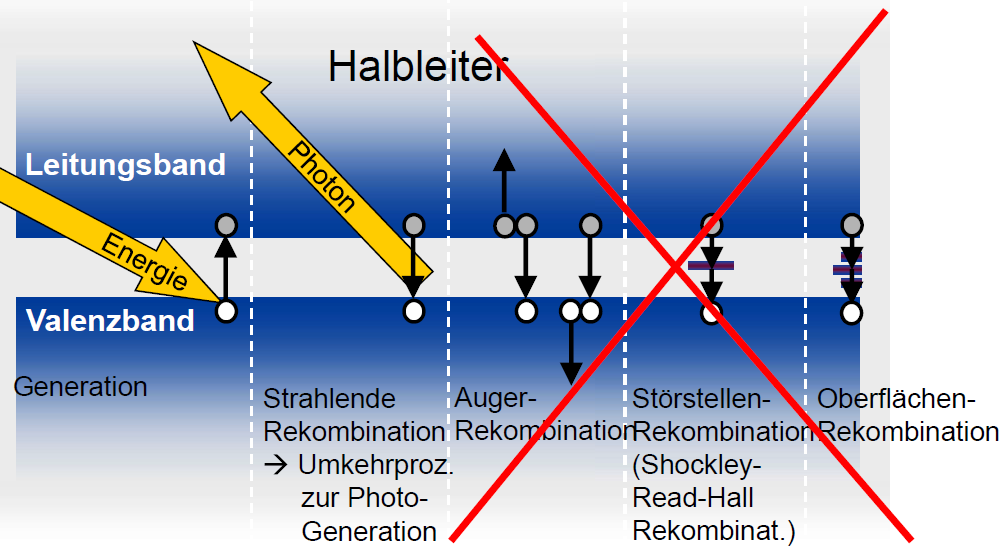
\includegraphics[width=0.5\textwidth]{Kapitel/Kap11/rekombination.png}
		\caption{Rekombination an LEDs}
		\label{11_rekombination}
	\end{figure}
	
	\subsubsection{Verschiedene Farben}
	
	Die Farbe wird durch die abgestrahlte Energie, und somit durch die Größe der Bandlücke bestimmt. Die Wellenlänge zu einer bestimmten Energie lässt sich mit folgender Formel berechnen:\\
	$\lambda(E_g) = \frac{hc}{E_g} = \frac{1240nm}{E_g}$\\
	Die Energie wird wie auch die Bandlücke in Elektronenvolt angegeben. Sie ist abhängig vom Halbleitermaterial (\ref{11_farben}).
	
	\begin{figure}
		\centering
		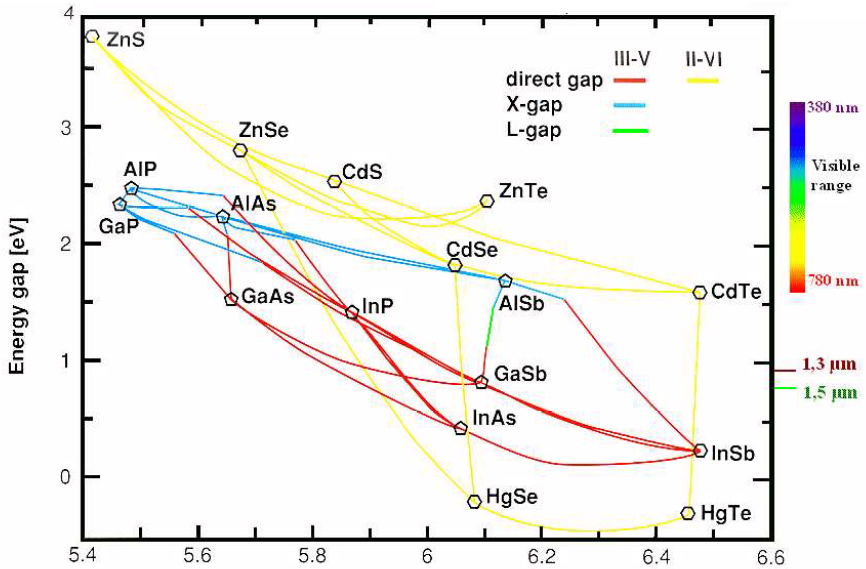
\includegraphics[width=0.5\textwidth]{Kapitel/Kap11/farben.png}
		\caption{Unterschiedliche Halbleiter und ihre Farben}
		\label{11_farben}
	\end{figure}
	
	\subsubsection{Weiße Dioden}
	
	Weißes licht kann auf mehrere Arten erstellt werden. Weißes licht ist eine Mischung aus mehreren Anteilen. So benötigt man für weißes Licht ein sehr Breitbandiges Lichtspektrum. Eine LED war jedoch gerade dafür bekannt relativ monochromatisch zu arbeiten. Zum einen kann eine Mischung aus RGB Anteilen stattfinden. Damit dies gut funktioniert müssen die einzelnen Farblichquelle sehr nahe beieinander liegen. Deshalb werden diese oftmals direkt in einem Bauteil zusammengefasst. Eine weitere Möglichkeit besteht daran, eine LED zu nehmen und das licht durch aufgelegte Stoffe zu beeinflussen. So kann eine UV-LED mit 3 unterschiedlichen Fluoreszenz-Farbstoffen in die RGB Anteile verschoben werden, die dann zusammen weißes licht ergeben. Eine billigere Variante Verwendet eine blaue LED, die mit nur einem Farbstoff ein gelb dazu mischt. Das hierbei entstehende Licht ist meistens sehr kalt, da der Blauanteil überwiegt.

	Generell lässt sich jedoch erkennen, dass sich die Farbspektren der unterschiedlichen Leuchtmittel stark unterscheiden (\ref{11_spektrum}). So hat eine Glühlampe einen sehr hohen Anteil an IR-Strahlung, was zu einem warmen (Wortwörtlich) Licht führt. Das Tageslicht enthält weniger rot, dafür mehr blau. Eine Leuchtstofflampe erzeugt nur einige genau definierte Spektralanteile. 
	
	\begin{figure}
		\centering
		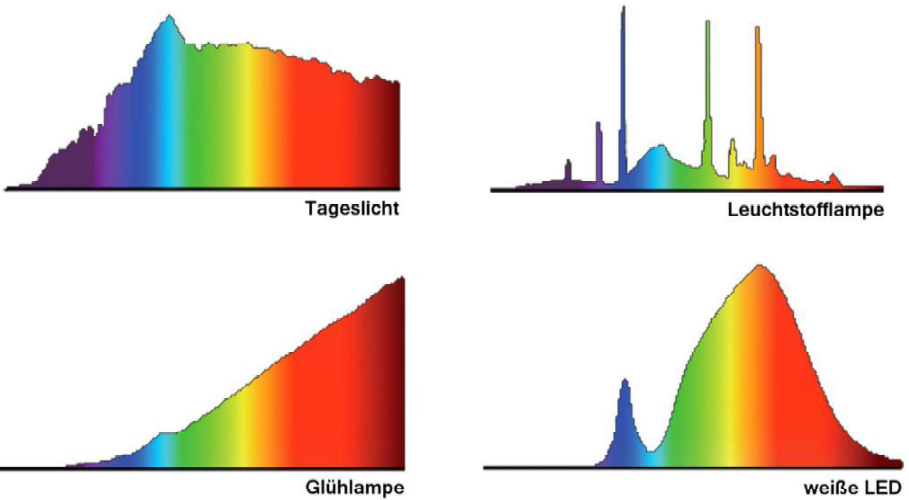
\includegraphics[width=0.5\textwidth]{Kapitel/Kap11/spektrum.png}
		\caption{Das Licht der Sonne, einer Leuchtstofflampe, einer Glühlampe und einer LED im Vergleich}
		\label{11_spektrum}
	\end{figure}
	
\subsection{Laser}
\todo{machen}
	\subsubsection{Funktionsprinzip (stimulierte Emission, Pumpen, beteiligte Energieniveaus, ...)}
	
	\subsubsection{Resonatoren}
	\subsubsection{Halbleiterlaser (Prinzipeller Aufbau, VCSEL, ...)}


\todo{Fragen aus Own Clowd zuordnen}
\todo{Gruppenübungs-Inhalte ergänzen}